\documentclass[border=4pt]{standalone}
\usepackage{tikz}
\usetikzlibrary{arrows.meta,positioning}
\usepackage[T1]{fontenc}
\usepackage{lmodern}

\definecolor{nb}{HTML}{3D4574}
\definecolor{rb}{HTML}{B83232}
\definecolor{sub}{HTML}{C8CCDF}

\tikzset{
  mbox/.style={
    rectangle, rounded corners=6pt, draw=none, fill=nb,
    text=white, font=\bfseries\scriptsize,
    minimum height=0.95cm, minimum width=2.05cm, text width=1.95cm,
    align=center, inner sep=2.5pt
  },
  rbox/.style={mbox, fill=rb},
  arr/.style={-Stealth, line width=1.1pt, black}
}

\begin{document}
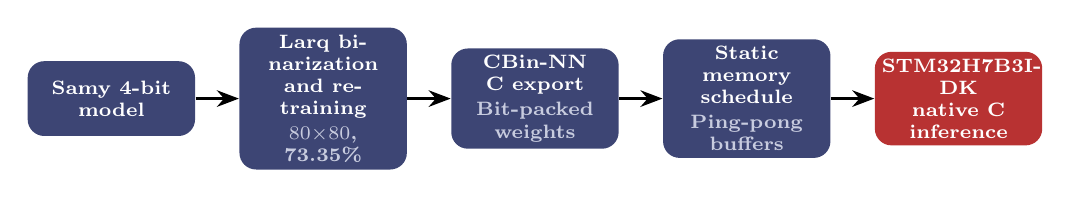
\begin{tikzpicture}[node distance=0.55cm]

\node[mbox] (samy) {Samy 4-bit\\model};

\node[mbox, right=of samy] (bin)
  {Larq binarization\\and retraining%
  \\[1pt]\textcolor{sub}{\scriptsize $80{\times}80$, 73.35\%}};

\node[mbox, right=of bin] (cbin)
  {CBin-NN C export%
   \\[1pt]\textcolor{sub}{\scriptsize Bit-packed weights}};

\node[mbox, right=of cbin] (mem)
  {Static memory\\schedule%
   \\[1pt]\textcolor{sub}{\scriptsize Ping-pong buffers}};

\node[rbox, right=of mem] (stm)
  {STM32H7B3I-DK\\native C inference};

\draw[arr] (samy) -- (bin);
\draw[arr] (bin) -- (cbin);
\draw[arr] (cbin) -- (mem);
\draw[arr] (mem) -- (stm);

\end{tikzpicture}
\end{document}